\section{Convergence of Random Variables}
We clarify the relationship between different modes of converges in the Venn diagram below. Note that these inclusions can be checked through the reference \textit{Counterexamples in Probability} by Jordan M. Stoyanov. 
\begin{center}
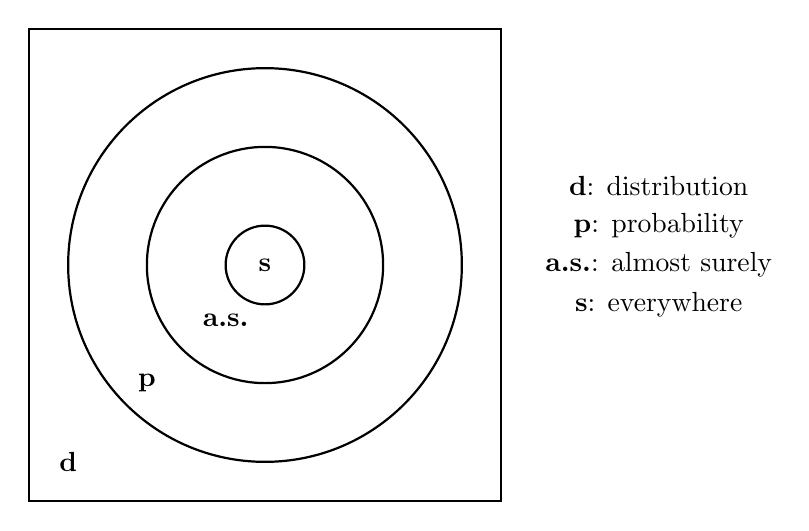
\begin{tikzpicture}
    \draw[thick] (-3,-3) rectangle (3,3);
    \draw[thick] (0,0) circle (2.5);
    \draw[thick] (0,0) circle (1.5);
    \draw[thick] (0,0) circle (0.5);
    \node at (-2.5,-2.5) {\textbf{d}};
    \node at (-1.5,-1.5) {\textbf{p}};
    \node at (-0.5,-0.7) {\textbf{a.s.}};
    \node at (0,0) {\textbf{s}};
    \node at (5,1) {\textbf{d}: distribution};
    \node at (5,0.5) {\textbf{p}: probability};
    \node at (5,0) {\textbf{a.s.}: almost surely};
    \node at (5,-0.5) {\textbf{s}: everywhere};
\end{tikzpicture}
\end{center}
We now prove some important lemmas regarding convergence of random variables that are useful for solving the problems above.
\begin{definition}
    Let $\xi_1,\xi_2,\ldots$ be a sequence of random variables. We say that this sequence Cauchy converges in probability if for any $\epsilon > 0$, 
    \[
    \lim_{n,m\to\infty} \Pr\left[ |\xi_m - \xi_n| \geq \epsilon\right] = 0.
    \]
\end{definition}

\begin{lemma}
    If $\xi_1,\xi_2,\ldots$ is a sequence of random variables that Cauchy converges in probability, then there exists a random variable $\xi$ that is finite almost everywhere such that $\xi_1,\xi_2,\ldots$ converges in probability. 
\end{lemma}
\begin{proof}
    
\end{proof}